\documentclass[12pt, a4paper]{article}
    \usepackage[utf8]{inputenc}
    %\usepackage[english, spanish]{babel}
    %\usepackage{fullpage} % changes the margin
    \usepackage{graphicx} 
    \usepackage{enumitem} 
    \usepackage{chngcntr}
    \counterwithin{figure}{section}
    \renewcommand{\thesection}{\arabic{section}} 
    \renewcommand{\thesubsection}{\thesection.\arabic{subsection}}
    \renewcommand{\baselinestretch}{1.5}

    \usepackage{amsmath}
    \usepackage{mathptmx}
    \usepackage[spanish, es-tabla]{babel} %es-tabla añadido
    \usepackage{amssymb}
    \usepackage{makeidx}
    \usepackage{float}
    \pagenumbering{arabic}
    \usepackage[left=25mm, right=25mm, top=25mm, bottom=25mm]{geometry}

    \usepackage[backend=biber]{biblatex}
    \bibliography{referencias}

\begin{document}

    \begin{titlepage}
        \centering
        {\scshape\Large Universidad Central de Venezuela \par}
        {\scshape\Large Facultad de ingeniería \par}
        {\scshape\Large Escuela de ingeniería Eléctrica \par}
        {\scshape\Large Departamento de Electrónica, Computación y Control \par}

        \vspace{6cm}
        {\Large\bfseries Pre-Laboratorio 5 : Polarización del JFET\par}
        \vspace{6cm}

        \vfill
        \begin{flushright}
            Estudiante:\par
            Santana Ricardo C.I.:29571461 \par
            \vspace{1cm}  
        \end{flushright}
        \vfill
        {\large \today \par}
    \end{titlepage}

    \section{Introducción}

    Existen diversos tipos de transistores con distintas aplicaciones, de los cuales cabe señalar el transistor de efecto de campo (FET), el cual controla la corriente que circula por uno de sus pines a través del voltaje aplicado entre sus otros dos terminales, a diferencia del BJT que controla la corriente respecto a otra corriente; por tal motivo el FET suele utilizarse en los circuitos como amplificador y como interruptor.

    Sin importar el tipo de FET, sea canal N o canal P, cuenta con tres terminales denominados puerta (Gate), drenador (Drain) y surtidor (Source). Cada uno cuenta con su característica de transferencia específicas y datos particulares que permitiran polarizar el transistor y operarlo en la zona deseada, las más comunes son el voltaje de Pinch-Off y la corriente de dreandor con $V_{GS} = 0$. 

    \newpage

    \section{Objetivos}

    \subsection{Objetivo General}
    \begin{itemize}
        \item Analizar el modo de operacion de un transistor JFET canal n. 
    \end{itemize}

    \subsection{Objetivos Específicos}
    \begin{itemize}
        \item Estudiar la polarización de un JFET de canal n.
        \item Reconocer y trabajar con la característica de transferencia y la característica de salida de un JFET de canal n.
    \end{itemize}

    \newpage

    \section{Marco Teórico}

    \subsection{Transistor FET.}

    El transistor de efecto de campo FET (Field Effect Transistor), es un dispositivo semiconductor de portadores mayoritarios, de tres terminales, cuya operación depende de la aplicación de un campo eléctrico para el control de las corrientes, esto es, el FET es una fuente de corriente controlada por tensión.Los FET pueden plantearse como resistencias controladas por diferencia de potencial. Tienen tres terminales, denominadas Puerta (gate), Drenador (drain) y Fuente (source). La puerta es la terminal equivalente a la base del BJT. El transistor de efecto de campo se comporta como un interruptor controlado por tensión, donde el voltaje aplicado a la puerta permite hacer que fluya o no corriente entre drenador y fuente.Así como los transistores bipolares se dividen en NPN y PNP, los de efecto de campo o FET son también de dos tipos: canal N y canal P.

    \begin{figure}[h!]
        \centering
        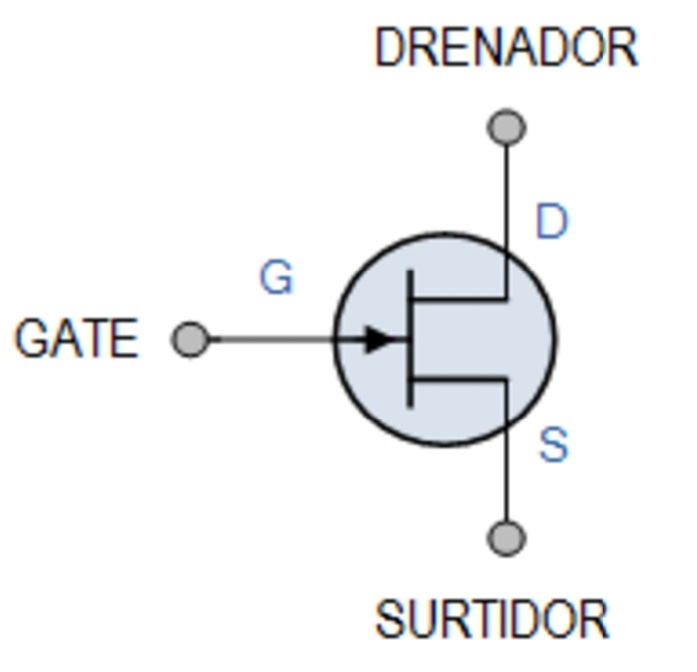
\includegraphics[height=5cm\textwidth]{fetn.jpg}
        \caption{Transistor FET canal n}
        \label{fig:t1}
    \end{figure}

    \begin{figure}[h!]
        \centering
        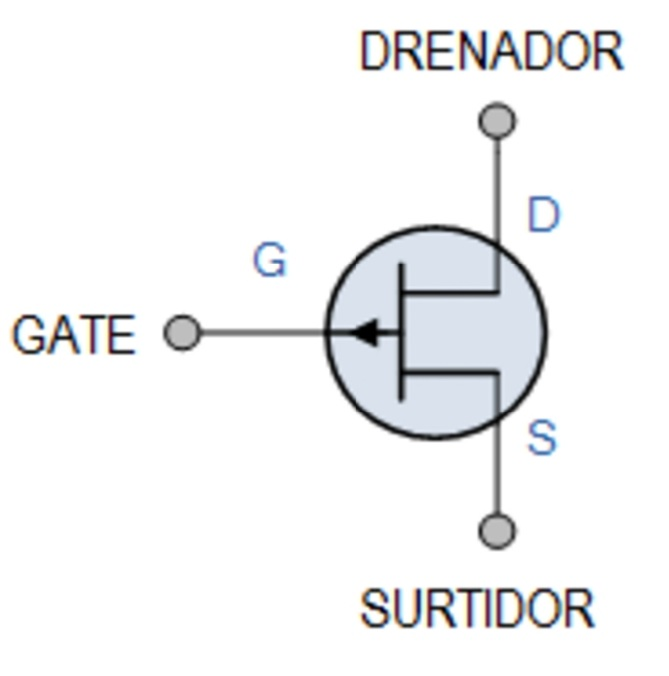
\includegraphics[height=5cm\textwidth]{fetp.jpg}
        \caption{Transistor FET canal p}
        \label{fig:t2}
    \end{figure}

    \subsection{Polarización FET}

    El modo normal de polarización de un FET de canal N requiere que la tensión entre puerta y fuente sea negativa ($V_{GS} < 0$) mientras que la tensión entre Drenador y Fuente tiene que ser positiva ($V_{DS} > 0$).

    \begin{figure}[h!]
        \centering
        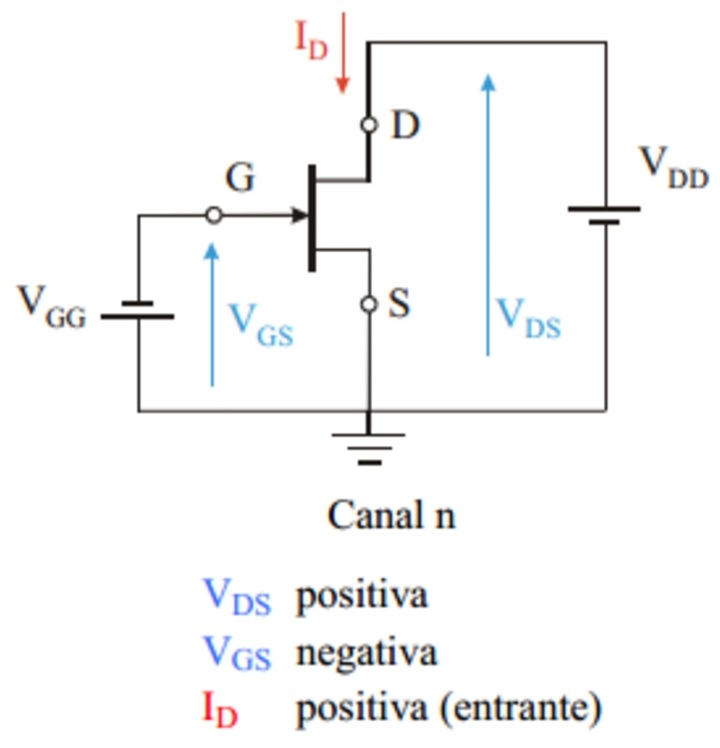
\includegraphics[height=5cm\textwidth]{polarizacionfet.jpg}
        \caption{Polarización del FET}
        \label{fig:t3}
    \end{figure}

    \subsection{Tipos de transistores de efecto de campo FET.}

    Hay muchas formas de definir los diferentes tipos de FET disponibles. Los diferentes tipos significan que, durante el diseño del circuito electrónico, hay una elección del componente electrónico adecuado para el circuito. Al seleccionar el dispositivo correcto, es posible obtener el mejor rendimiento para el circuito dado.
    
    Los FET pueden clasificarse de varias formas. Hay muchos tipos diferentes de FET en el mercado para los que existen varios nombres. Algunas de las categorías principales son:

    \begin{itemize}
        \item JFET
        \item MOSFET
    \end{itemize}

    \subsection{Transistor JFET.}

    El transistor de efecto de campo de unión o JFET es un dispositivo semiconductor unipolar de tres terminales.

    Es básicamente una barra semiconductora N o P (canal), en unión con otros dos semiconductores contrarios al tipo del canal. Si el canal es de semiconductor N, los otros 2 semiconductores serán P o si el canal es de semiconductor P, los otros 2 semiconductores serán N. Tiene 3 contactos unidos a los semiconductores por contactos óhmicos, El drenador (D) y la fuente (F) en los extremos del canal, y otra patilla llamada Puerta o Gate (G)en uno de los otros 2 semiconductores.

    \subsection{Estructura del JFET}

    La ruta de corriente entre estos dos terminales (fuente y drenador) se denomina "canal", que puede estar hecho de un material semiconductor tipo P o tipo N.

    \begin{itemize}
        \item Si el canal es del tipo semiconductor N se llama JFET de canal N (las otras patitasas serán P).
        \item Si el canal es del tipo semiconductor P se llaman JFET de canal P (las otras patillas serán N).
    \end{itemize}

    \subsection{Funcionamiento del JFET}

    En un JFET de canal N tenemos una 2 uniones PN entre el gate (G), que es semiconductor P y la fuente (N) que es el canal y la otra entre el otro semiconductor P y el canal. Si esta unión PN la polarizamos inversamente, la unión PN entre G y el canal tenemos la tensión $V_{GS}$. 
    
    Al aumentar esta tensión aumentará la zona de agotamiento y por lo tanto disminuirá el ancho del canal, lo que hace que tendrá más resistencia al paso de la corriente. La zona de agotamiento a veces también se llama zona de deplexión. Si disminuye el canal, la corriente entre el drenador (D) y la fuente (S) disminuye.

    \subsection{Voltaje de “pinch off” }

    El voltaje de Pinch off es el voltaje que se aplica a la puerta o compuerta de un transistor JFET para estrangular el canal y reducir la corriente de drenaje a un nivel muy bajo. El voltaje de Pinch off también determina la transición del transistor de la región lineal a la región de saturación, donde el transistor actúa como una fuente de corriente constante. El voltaje de Pinch off depende del tipo y las dimensiones del canal.

    \subsection{Regiones de operación del JFET}

    \subsubsection{JFET en región de corte}

    En esta región la intensidad entre drenador y fuente es nula (ID=0). En este caso, la tensión entre puerta y fuente es suficientemente negativa que las zonas de inversión bloquean y estrangulan el canal cortando la corriente entre drenador y fuente.

    En las hojas técnicas se denomina a esta tensión como de estrangulamiento o pinch-off y se representa por VGS (off) o Vp.

    \subsubsection{JFET en región lineal}

    En esta región, el JFET se comporta como una resistencia no lineal que es utilizada en muchas aplicaciones donde se precise una resistencia variable controlada por tensión.

    \subsubsection{JFET en región de saturación}

    En esta región, de similares características que un BJT en la región lineal, el JFET tiene unas características lineales que son utilizadas en amplificación.

    Se comporta como una fuente de intensidad controlada por la tensión VGS cuya ID es prácticamente independiente de la tensión VDS. La ecuación que relaciona la ID con la VGS se conoce como ecuación cuadrática o ecuación de Schockley que viene dada por

    $$I_D = I_{DSS}\left( 1-{V_{GS} \over V_P}\right) ^2$$

    donde $V_p$ es la tensión de estrangulamiento y la $I_{DSS}$ es la corriente de saturación. Esta corriente se define como el valor de $I_D$ cuando $V_{GS}=0$, y esta característica es utilizada con frecuencia para obtener una fuente de corriente de valor constante ($I_{DSS}$).

    Esta relación junto a las características del JFET permiten obtener gráficamente el punto estático de operaciones Q del transistor en la región de saturación. La figura 4 muestra la representación gráfica de este punto Q y la relación existente en ambas curvas, la característica de transferencia y, las cuales permiten determinar el punto de polarización de un transistor utilizando métodos gráficos.

    \begin{figure}[h!]
        \centering
        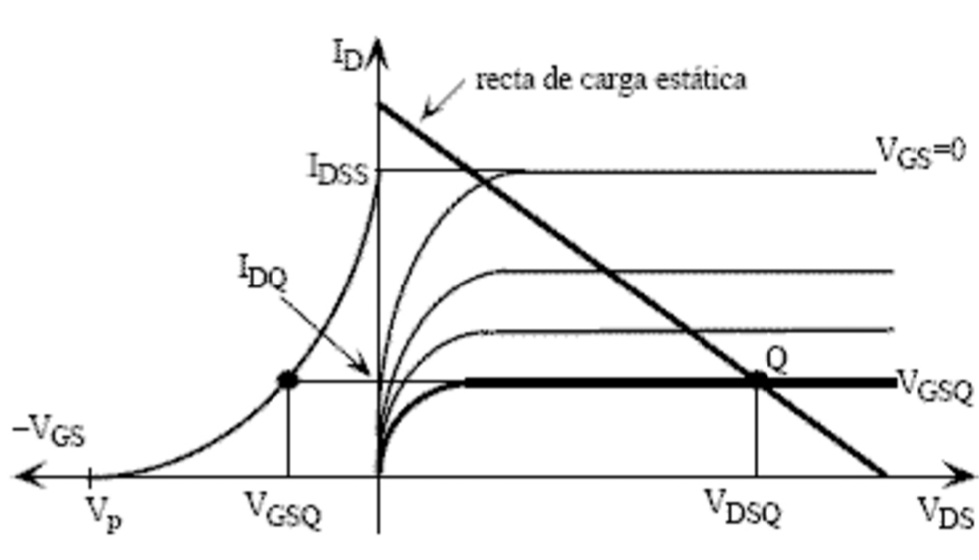
\includegraphics[height=5cm\textwidth]{curvafet.jpg}
        \caption{Curva característica de transferencia y el punto de operaciones Q}
        \label{fig:t4}
    \end{figure}

    \subsubsection{FET en región de ruptura}

    Una tensión alta en los terminales del JFET puede producir ruptura por avalancha a través de la unión de puerta. Las especificaciones de los fabricantes indican la tensión de ruptura entre drenaje y fuente con la puerta cortocircuitada con la fuente; esta tensión su valor está comprendido entra 20 y 50V. Las tensiones de polarización nunca deben superar estos valores para evitar que el dispositivo se deteriore.

    \newpage

    \section{Metodología}

    \subsection{Trabajo Previo al Laboratorio}

    \begin{enumerate}
        \item \label{p11}	Determine el punto estático de operación para el circuito de la Figura \ref{fig:cir1}. Para el valor de $I_{DSS}$ y Vp, deben obtenerlo del manual del fabricante según el transistor a utilizar.
        \item \label{p12}	Obtenga la tensión en cada uno de los terminales del JFET: tensión en el Drenador ($V_D$), tensión en la Puerta ($V_G$) y la tensión en el Surtidor ($V_S$).
    \end{enumerate}

    \begin{figure}[h!]
        \centering
        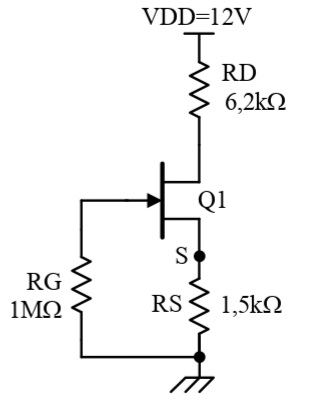
\includegraphics[height=5cm\textwidth]{circuito1.jpg}
        \caption{Polarización del JFET canal n.}
        \label{fig:cir1}
    \end{figure}

    \subsection{Trabajo de Laboratorio}

    \begin{enumerate}
        \item \label{p21}	Para el circuito de la Figura \ref{fig:cir1}, mida la tensión en el Drenador (VD), tensión en la Puerta ($V_G$) y la tensión en el Surtidor ($V_S$). Determine el punto estático de operación: la tensión Drenador-Surtidor ($V_D$S) haciendo $V_D-V_S$ de los valores medidos y la corriente de Drenador ($I_D$) de manera indirecta haciendo $(V_{DD}-V_D)/R_D$; para RD emplear su valor nominal.
        \item \label{p22}	Para el circuito de la Figura \ref{fig:cir2}, varíe el potenciómetro de hasta conseguir el punto de estático de operación. Anote las mediciones.
        \item \label{p23} 	Varíe el potenciómetro hacia un sentido para conseguir una variación de $0.1V$ en la tensión del Drenador ($V_D$) con respecto al medido en el punto \ref{p22}, anote el valor y mida la tensión en los otros terminales del transistor.
        \item \label{p24} 	Siga variando el potenciómetro en el mismo sentido que el punto \ref{23} para obtener variaciones de 0,1V en la tensión del Drenador (VD) hasta llegar al extremo del potenciómetro. En cada variación mida las tensiones en cada uno de los terminales del transistor. Realice una tabla.
    \end{enumerate}

    \begin{figure}[h!]
        \centering
        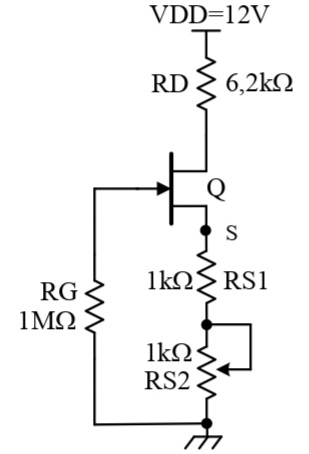
\includegraphics[height=5cm\textwidth]{circuito2.jpg}
        \caption{Variación en la Polarización del JFET.}
        \label{fig:cir2}
    \end{figure}

    \newpage

    \section{Cálculos prévios}

    Se trabajará con el transistor FET canal n MPF102, el cual posee las siguientes especificaciones:
    
    \begin{table}[h!]
        \centering
        \caption{Características del transistor MPF102} %nombre de la tabla
        \label{tab:K61-Y} %indice de la tabla
        \begin{tabular}{c}
            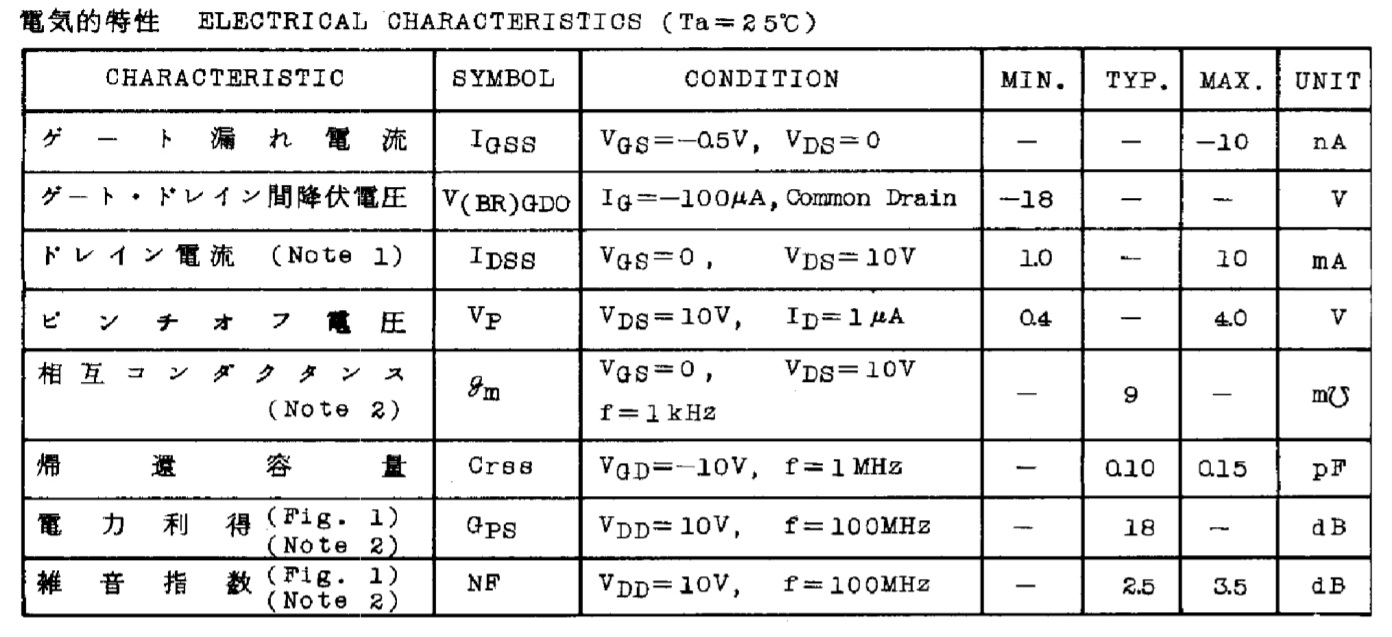
\includegraphics[width=16cm\textwidth]{K61-Y.jpg} \\
        \end{tabular}
    \end{table}
    
    de las cuales se deduce por promediación que:

    $V_P = -2.2V$

    $I_{DSS} = 5mA$

    Entonces analizando el siguiente circuito, para encontrar el punto de operación $Q(V_{DSQ},I_{DQ})$

    \begin{figure}[h!]
        \centering
        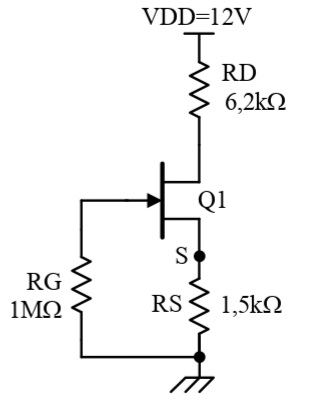
\includegraphics[height=5cm\textwidth]{circuito1.jpg} \par
        Figura \ref{fig:cir1}. Polarización del JFET canal n.
    \end{figure}

    Se tiene un JFET autopolarizado. Esto es debido a que la corriente circulando por $R_G$ es cero y, por tanto, toda la corriente ($I_D$) que entra por el drenador D sale por la fuente S.

    Analizando la malla relacionada al circuito de la compuerta con $I_G = 0$,

    $$V_{GS} = -I_DR_S \rightarrow I_D = -{V_{GS} \over R_S}$$

    \begin{equation}
        \label{eq1}
        I_D = -{V_{GS} \over R_S}
    \end{equation}

    Conociendo la características de transferencia de un JFET que relaciona $V_{GS}$ e $I_D$

    \begin{equation}
        \label{eq2}
        I_D = I_{DSS}\left( 1-{V_{GS} \over V_P}\right) ^2
    \end{equation}

    Entonces

    $$I_{DQ} = I_{DSS}\left( 1-{V_{GSQ} \over V_P}\right) ^2 = -{V_{GSQ} \over R_S}$$

    buscando $V_{GSQ}$
    
    \begin{equation}
        \label{eq3}
        \begin{split}
            I_{DSS}\left( 1-{V_{GSQ} \over V_P}\right) ^2  & = -{V_{GSQ} \over R_S} \\
            1 - 2{V_{GSQ} \over V_P} + ({V_{GSQ} \over V_P})^2  & = -{V_{GSQ} \over I_{DSS}R_S} \\
            1 - 2{V_{GSQ} \over V_P} + {V_{GSQ}^2 \over V_P^2} + {V_{GSQ} \over I_{DSS}R_S} & = 0 \\
            {1 \over V_P^2}V_{GSQ}^2 + \left({1 \over I_{DSS}R_S} - {2 \over V_P}\right)V_{GSQ} + 1 & = 0 \\
        \end{split}
    \end{equation}

    Reemplazando valores conocidos en \eqref{eq3} y resolviendo ecuación de segundo grado

    \begin{split}
        {1 \over V_P^2}V_{GSQ}^2 + \left({1 \over I_{DSS}R_S} - {2 \over V_P}\right)V_{GSQ} + 1 & = 0 \\
        {1 \over (-2.2V)^2}V_{GSQ}^2 + \left({1 \over (5mA)(1.5k\Omega)} - {2 \over (-2.2V)}\right)V_{GSQ} + 1 & = 0 \\
        {25 \over 121}V_{GSQ}^2 + {172 \over 165}V_{GSQ} + 1 & = 0 \\
    \end{split}

    $$V_{GSQ} = -1.29V$$

    \begin{figure}[h!]
        \centering
        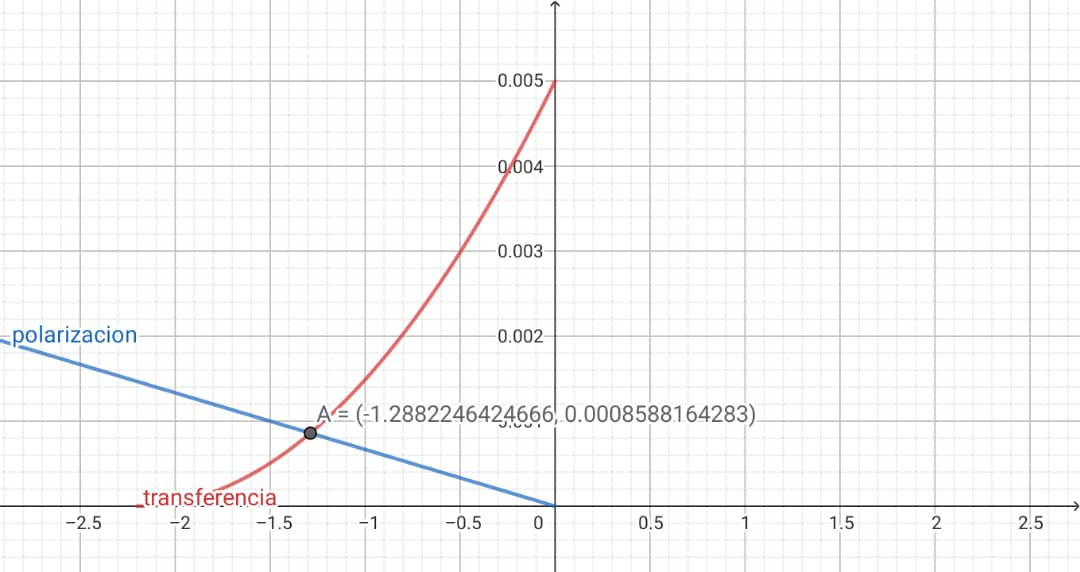
\includegraphics[height=5cm\textwidth]{graficoQ.jpg}
        \caption{Intersección de las ecuaciones \eqref{eq1} y \eqref{eq2}}
        \label{fig:vgsq}
    \end{figure}

    Sustiyendo en \eqref{eq1}

    $$I_{DQ} = -{V_{GSQ} \over R_S} = -{(-1.29V) \over 1.5k\Omega} = 0.86mA$$

    Analizando malla relacionada al drenador

    $$V_{DD} = I_DR_D + V_{DS} + I_DR_S$$

    Particularizando para calcular $V_{DSQ}$

    \begin{equation}
        \label{eq4}
        \begin{split}
            V_{DD} & = I_{DQ}R_D + V_{DSQ} + I_{DQ}R_S \\
            I_{DQ}R_D + V_{DSQ} + I_{DQ}R_S & = V_{DD} \\
            V_{DSQ} & = V_{DD} - I_{DQ}(R_D + R_S)
        \end{split}
    \end{equation}
    
    Reemplazando valores en \eqref{eq4}

    $$V_{DSQ} = 12V - 0.86mA(6.2 + 1.5)k\Omega = 5.378V$$

    Punto de operacion

    $$Q : (5.378V, 0.86mA)$$

    Entonces el transistor se encuentra en zona de saturación
    
    Como $I_G = 0$, entonces no hay caida de tensión en $R_G$ y $V_G = 0$

    $V_S = - V_{GS} = 1.29V$

    $V_{DS} = V_D - V_S \rightarrow V_D = V_{DS} + V_S = 5.378V + 1.29V = 6.668V$

    \begin{table}[h!]
        \centering
        \caption{Voltajes teoricos en Puerta, Drenador y Fuente}
        \label{tab:vteorico} 
        \begin{tabular}{|c|c|c|} \hline
            V_G [V] & V_D [v] & V_S [v] \\ \hline
            0 & 6.668 & 1.290 \\ \hline
        \end{tabular}
    \end{table}

    \newpage

    \section{Materiales e Instrumentos}

    %hay que realizar tablas

    \begin{itemize}
        \item Transistor FET canal n 2SK61
        \item Resistencia de carbon de $6.2k\Omega$  serie del $5\%$ y potencia de $1/4$ W.
        \item Resistencia de carbon de $1.5k\Omega$  serie del $5\%$ y potencia de $1/4$ W.
        \item Resistencia de carbon de $1M\Omega$  serie del $5\%$ y potencia de $1/4$ W.
        \item Resistencia de carbon de $1k\Omega$  serie del $5\%$ y potencia de $1/4$ W.
        \item Potenciometro Preset de $1k\Omega$  serie del $10\%$
    \end{itemize}

\end{document}